\section{A New Real-time POV}

\subsection{System Architecture}
\begin{frame}{System Architecture}
	\textcolor{blue}{Assumption:\\ \tab{} $\text{同時 k 個 server,同時回傳相同錯誤結果的機率} \approx 0$}
	\begin{center}
		\alert{Service Providers are Independent Cloud}
		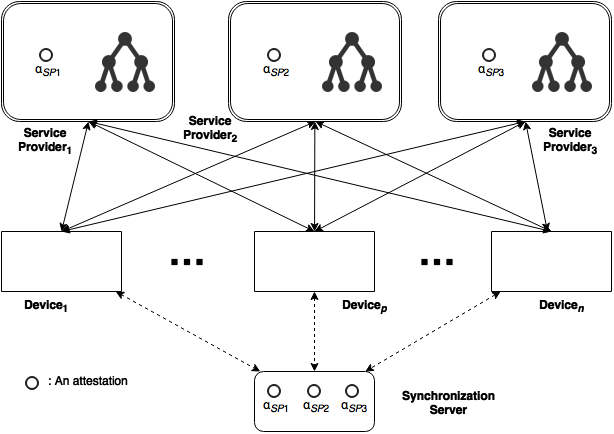
\includegraphics[height=.7\textheight]{wei_chih}
	\end{center}
\end{frame}

\begin{frame}{Comparison}
	\begin{itemize}
		\item \textcolor{blue}{Pros}
			\begin{enumerate}
				\item Device 節省了儲存 Merkle tree 的空間
                \item Device 不需要計算新的 Roothash 將會節省時間
				\item 每一次更新資料都會即時的備份
				\item 不會有之前的 Worst-case
			\end{enumerate}
		~\\
		\item \textcolor{red}{Cons}
			\begin{enumerate}
				\item 需要傳送多份 Request, 處理多份 Response
                \item 需要使用較多的 Service Provider
			\end{enumerate}
	\end{itemize}
\end{frame}

\subsection{System Flowchart}
\begin{frame}{System Flowchart}
	\begin{center}
		\resizebox{!}{.7\textwidth}
		{%
			\begin{tikzpicture}[node distance=2cm]
				% Define flow charts' component
				\node (init) [process] {Initial};
				\node (lock) [process, below of=init] {Lock};
				\node (twostep) [process, below of=lock] {Request \& Response};
				\node (twostep_left) [process, left of=twostep, xshift=-2cm] {Request \& Response};
				\node (twostep_right) [process, right of=twostep, xshift=2cm] {Request \& Response};
				\node (voting) [decision, below of=twostep] {Voting};
				\node (store) [process, below of=voting, yshift=-0.5cm] {Store ACK};
				\node (update) [io, below of=store, align=center] {File \\ Transmit};
				\node (auditing) [process, right of=store, xshift=2.5cm] {Auditing};
				\node (unlock) [process, left of=store, xshift=-4cm] {Unlock};

				% Define flow charts' link
				\path [line](init) -- (lock);
				\path [line](lock) -- (twostep);
				\path [line](lock) -- (twostep_left);
				\path [line](lock) -- (twostep_right);
				\path [line](twostep) -- (voting);
				\path [line](twostep_left) -- (voting);
				\path [line](twostep_right) -- (voting);
				\path [line](voting) -- node[anchor=east] {k個以上的}
									    node[anchor=west] {ACK相同} (store);
				\path [line](voting) -| node[anchor=west] {ACK不相同} (auditing);
				\path [line](store) -- (update);
				\path [line](store) -- (unlock);
				\path [line](unlock) |- (lock);
			\end{tikzpicture}%
		}
	\end{center}
\end{frame}

\subsection{Download \& Upload}
\begin{frame}{Download \& Upload}
	\centering
	\textcolor{blue}{\textbf{Request \& Response}}\\
	~\\
	~\\
	\begin{minipage}{.45\textwidth}
		\includegraphics[width=\textwidth]{2_step_handshake}
    \end{minipage}%
	\begin{minipage}{.55\textwidth}
    	\footnotesize
		\centering
		\begin{equation*} \label{eq1}
                \begin{split}
                        \textcolor{blue}{REQ}\ & =\ (OP,\ SN,\ [OP,\ SN]_{pri(D)}) \\
                        OP\ & =\ (TYPE,\ PATH,\ HASH) \\
                        SN\ & =\ Sequence\ Number
                \end{split}
        \end{equation*}
        \hrule{}
        \begin{equation*} \label{eq2}
                \begin{split}
                        \textcolor{red}{ACK}\ & =\ (RESULT,\ REQ,\\
                        & \tab{}\tab{}[RESULT,\ REQ]_{pri(S)}) \\
                        RESULT\ & =\ (roothash,\ filehash)
                \end{split}
        \end{equation*}
        \textcolor{red}{\textbf{collect ACKs and voting}}
    \end{minipage}%
\end{frame}

\begin{frame}{if Operation is UPLOAD}
	\centering
    ~\\
	\textcolor{blue}{\textbf{Servers Update Merkle tree}}\\
	~\\
	\begin{center}
		\includegraphics[height=.7\textheight]{update_merkle_tree}
	\end{center}
\end{frame}

\begin{frame}{File Transmit}
	\begin{center}
		\includegraphics[width=.9\textwidth]{file_transmit}
	\end{center}
\end{frame}

\subsection{Audit}
\begin{frame}{Audit}
	\begin{block}{}
		\centering
		device request $OP_i$,收到回傳的 $ACK_i$\\
		發現 $Server_p$ 的 ACK 有錯誤,因此向 $Server_p$ 稽核\\
		~\\
		device 向 $Server_p$ 索取 $MT_{i-1}$\\
		($MT_{i-1}$ 為執行 $OP_i$ 之前的 Merkle tree)
	\end{block}
	\begin{alertblock}{\encircle{1}\encircle{2} 兩點有一個出錯就能證明 $Server_p$ 出錯}
    	\alert{[證明 i 之前的動作都沒問題]}\\
		\encircle{1} device 檢查 $MT_{i-1}$ 的 roothash,應和 $ACK_{i-1}$ 中紀錄的相同\\
		~\\                   
        \alert{[證明第 i 個動作沒問題]}\\             
		\encircle{2} device 以 $OP_i$ 中的 hash value 來更新 $MT_{i-1}$,\\
					 \tab{}更新後的 roothash 應和 $Server_p$ 現在的 roothash 相同
	\end{alertblock}	
\end{frame}